\documentclass[conference]{acmsiggraph}

\title{A review on crowd simulation and rendering}

\author{Garoe Dorta-Perez}
\pdfauthor{Garoe Dorta-Perez}

\begin{document}

\maketitle

%% Required for all content. 

\section{Introduction}

%Include why crowd simulation is interesting in films and videogames????
Crowd simulation and rendering has been an active research area since 1987 
with the early work on bird flocks by \cite{Reynolds1987}, where it was
shown that by implementing some local rules in each entity a coherent
global behaviour could be achieved.
 
A crowd is much more than the collections of individuals
that form it. And as such the behaviour of the individuals could be
affected by other members of the crowd. As the numbers in the crowd
increase, the interrelations become quite computationally expensive.

The problem to be tackled has actually several differentiated areas. Firstly
there is a \textit{crowd generation problem}, a modeller needs easy to
use tools in order to set up a scene in which a crowd is present. Secondly,
the crowd is an evolving entity so there are \textit{crowd dynamics} to model,
which will govern the state of the crowd over time. Thirdly, the model should
be presented to the user, so a \textit{rendering} stage is needed.

\section{Classification}

A clear line can be drawn between real-time simulation (games)
and non real-time simulation (films). Since the requirements for this two types of simulation
are quite different and so are the techniques used in each area.

\subsection{Modelling Classifications}

In order to simulate crowd behaviour a number of approaches have been
proposed. As they shared certain similarities they can be divided 
using a common criteria such as time of the simulation and size
of the modelled crowd. So, in the time
axis we have short-term simulations, medium-term simulations and
long-term simulations. While in the size axis there are small,
medium and big size crowds. We can also use criteria according to
the type of model used for the agents in the crowd.

For small and medium crowds \textit{agent based} or \textit{entity based} systems are
commonly used. While for big size crowds the sheer number of individuals
makes it impractical, so the preferred method is to use \textit{flow based}
simulations.

\subsection{Rendering Classifications}

The different types of rendering techniques can be classified in the 
following groups: \textit{dynamically generated impostors} first used by  \cite{Aubel2000}, 
\textit{point-rendering} techniques \cite{Wand2002}, \textit{geometry baking} 
\cite{Ulicny2004} and \textit{dynamic} meshes \cite{Ciechomski2005}.

\begin{equation}
 \sum_{j=1}^{z} j = \frac{z(z+1)}{2}
\end{equation}

\begin{eqnarray}
x & \ll & y_{1} + \cdots + y_{n} \\
  & \leq & z
\end{eqnarray}

\section{Mayor milestones}

With the advent of programmable GPU there has been a shift of
general computation from the CPU to the GPU with substantial
increases in performance.

\subsection{Modelling milestones}

\subsection{Rendering milestones}

 LOD techniques, impostors, mesh decimation,
mesh subdivision, cloth simulation.

In order to lower the rendering cost ~\cite{pratt1997humans} TODO CHANGE TO CITED BY OTHER AUTHOR taken from ~\cite{Aubel1999} used a
LOD technique to be able to render crowds, however even though it 
achieved real time performance the realism of the models was quite
poor.


\begin{figure}[ht]
  \centering
  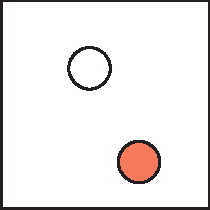
\includegraphics[width=1.5in]{images/samplefigure}
  \caption{Sample illustration.}
\end{figure}

\section{Conclusion}

\bibliographystyle{acmsiggraph}
\bibliography{template}
\end{document}
